\chapter{Future Work}\label{Sec:Future Work}

Many different adaptations, tests, and experiments have been left for the future due to lack of time (i.e. the experiments with real data are usually very time consuming, requiring even days to finish a single run). Future work concerns deeper analysis of particular mechanisms, new proposals to try different methods, or simply curiosity. There are some ideas that I would have liked to try during the description and the development of the fitness functions in Chapter 3. This thesis has been mainly focused on the use of EDAs for graph matching, and most of the fitness functions used to find the best result where obtained from the literature of adapted from these, leaving the study of fitness functions outside the scope of the thesis. The following ideas could be tested:
1. It could be interesting to consider the regions in the model and data images with different importance, depending on their size or their specific meaning with respect to the recognition process. This mechanism would for instance aid to distinguish in very complex problems which are the regions that are essential to be found, the ones that sometimes appear, and the ones that rarely do.
2. The way the model is constructed could be also changed: instead of using one typical image (prototype), it could be based on different images, in order to provide some information on the variability among the different images, and introduce it in the attributes. Unfortunately, in the type of images that we have taken as real examples the construction of a model from each image is a tedious task and no further study in this direction could be performed.

Try to avoid giving the synthesized data properties that makes it possible for a learning algorithm to distinguish synthesized from non-synthesized example such as if all the synthesized data comes from one of 20 car designs, or all the synthesized audio comes from only 1 hour of car noise. This advice can be hard to follow. 

\begin{figure}[ht]
	\begin{center}
		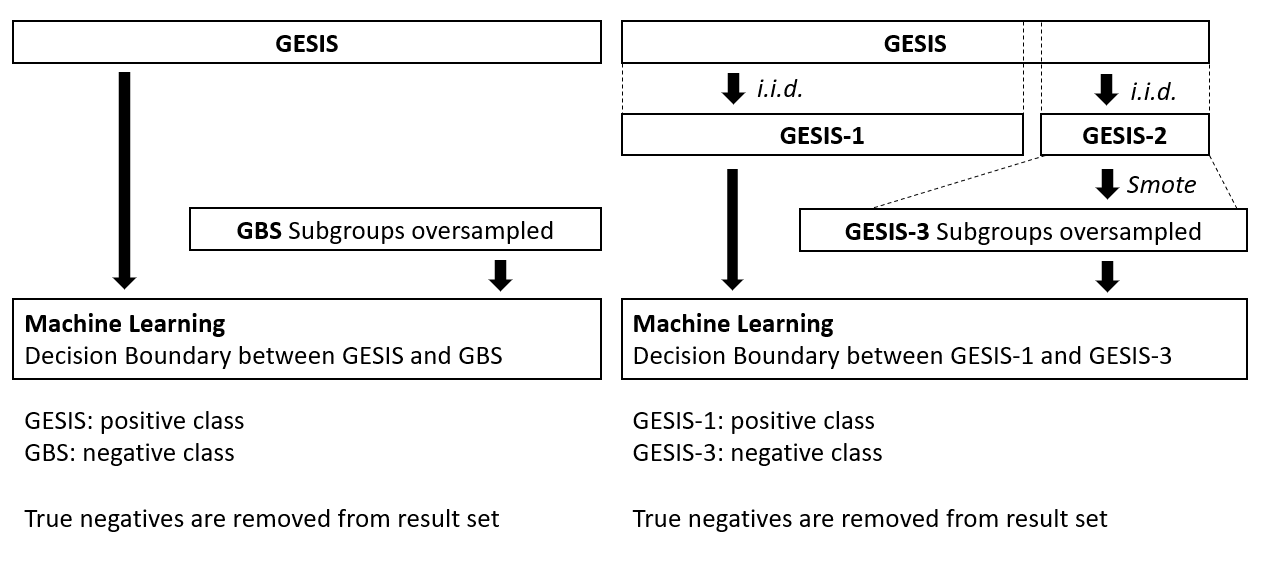
\includegraphics[scale=0.52,angle=0]{fig/procedure}
		\label{std}
	\end{center}
\end{figure}

%\begin{figure}[ht]
%	\begin{center}
%		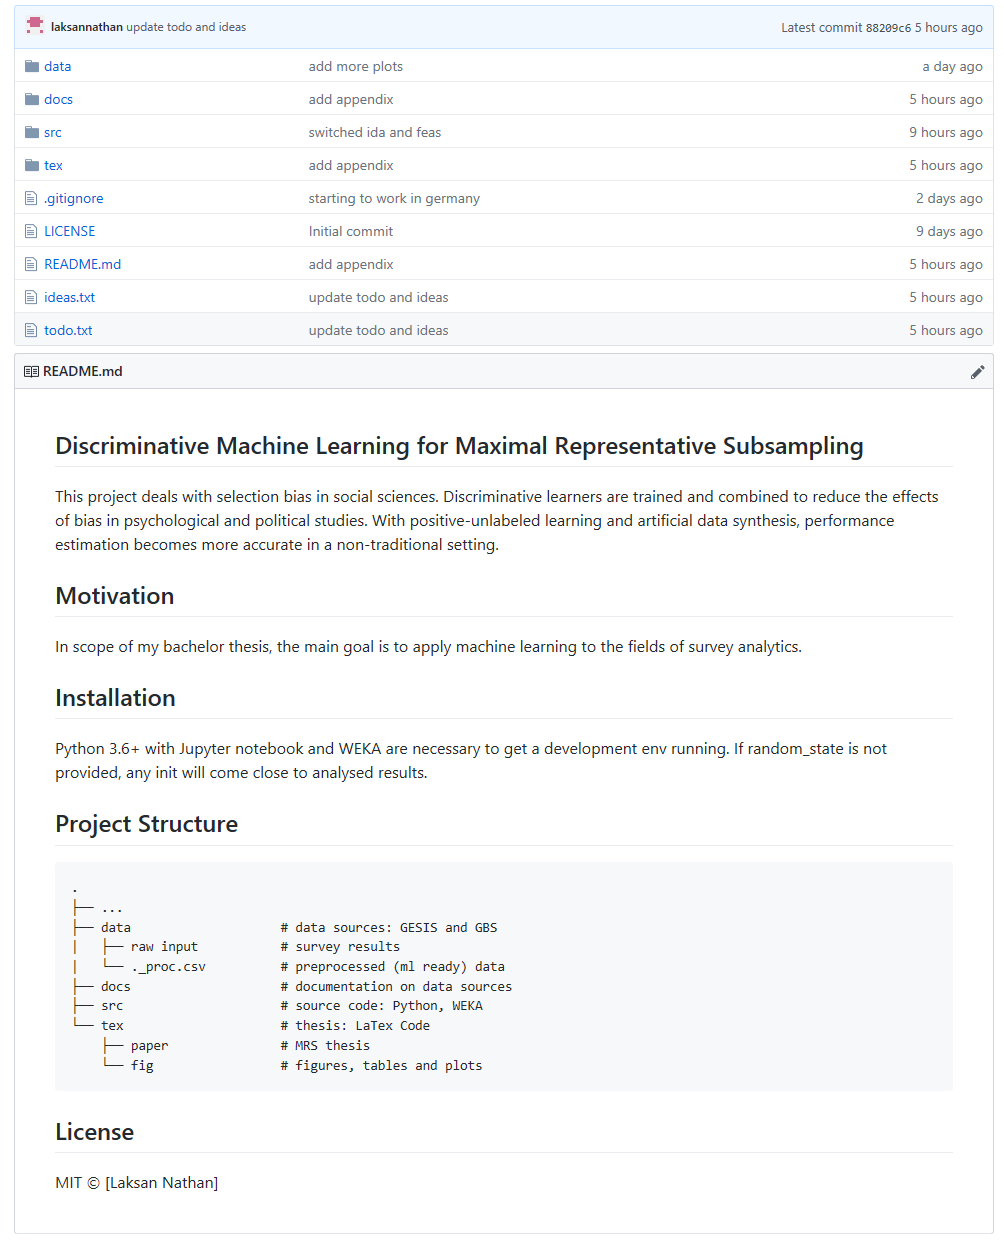
\includegraphics[scale=0.48,angle=0]{fig/github}
%		\label{std}
%\caption{The upper right triangular matrix  "erformances in predicting political participation. "Wahlabsicht" is therefore removed.}
%	\end{center}
%\end{figure}